\chapter{Introducción y nuevos objetivos}
\label{introduccción}
\section{Introducción}
En las últimas décadas el número de pasajeros de avión  ha aumentado exponencialmente, conllevando un aumento prácticamente similar del tráfico aéreo. Tan sólo en España en el año 2012 hubo 195 millones de viajeros en la red AENA, siendo el aeropuerto de Madrid-Barajas con 45 millones de viajeros el más visitado, seguido de cerca por el de Barcelona-El Prat con 35 millones. \\
\begin{figure}[H]
	\begin{center}
		\centering
		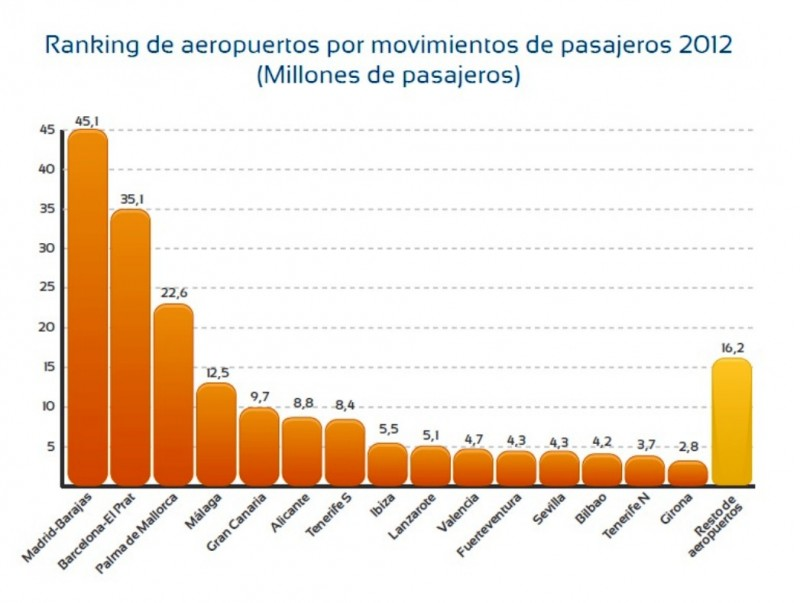
\includegraphics[width=0.8\textwidth]{./imagenes/introduccion/Ranking_de_aeropuertos_espayoles_por_pasajeros_horiz.jpg}
		\caption{Viajeros en aeropuertos españoles. \textit{Fuente: AENA}}
		\label{fig: Viajeros en aeropuertos españoles}
	\end{center}
\end{figure}
Este incremento del tráfico aéreo (actualmente hay de media 11.000 vuelos simultáneos por minuto) sumado a las limitaciones estructurales que tienen los aeropuertos para expandirse, ha ocasionado un importante problema de sobresaturación del espacio aéreo.\\
	

Para tratar de solucionar este problema, se creó en 1988 el Central Flow Management Unit (CDMU), entidad dependiente de EUROCONTROL cuyo contenido es centralizar y estructurar todo el tráfico europeo, al igual que hace el Air Traffic Control System Command Center en Estados Unidos. El CFMU trabaja a 3 niveles, según sea el espacio temporal sobre el que estén trabajando:
\begin{itemize}
	\item \textbf{Planificación táctica:} se realizan el mismo día para manejar las excepciones no previstas. Se trata de un modelo matemático diseñado para dar una respuesta muy rápida a una situación de excepción.
	\item \textbf{Planificación pre-táctica:} llevada a cabo con 2 días de antelación, se encarga de analizar el tráfico de los días previos, así como la previsión meteorológica.
	\item \textbf{Planificación estratégica: }se lleva a cabo cada 6 meses. En ella se elaboran los planes de vuelo para cada compañía y se asignan los recorridos disponibles para cada vuelo.
\end{itemize}


	
A pesar de todas estas estrategias de planificación, el conjunto histórico de datos, y las mejoras de previsión meteorológica, sigue existiendo un porcentaje importante de retrasos y cancelaciones. Según datos de EUROCONTROL, en el año 2016 un 20\% de los vuelos tuvieron un retraso superior a los 15 minutos:
\begin{figure}[h]
	\begin{center}
		\centering
		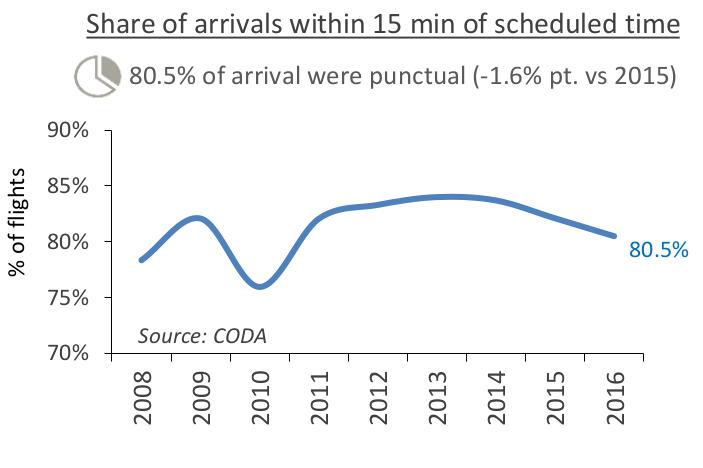
\includegraphics[width=0.8\textwidth]{./imagenes/introduccion/retrasos.png}
		\caption{Porcentaje retrasos en 2016. \textit{Fuente: EUROCONTROL}}
		\label{fig: Porcentaje retrasos en 2016}
	\end{center}
\end{figure}

Los motivos por los que un vuelo no llega en la hora prevista a su destino depende en gran medida de la zona geográfica que estudiemos: mientras que en Estados Unidos la mayor parte de los retrasos se debe a un cuello de botella que existe en sus aeropuertos, en Europa es la sobresaturación del espacio aéreo el principal problema, ya que hay un gran número de aeropuertos con mucho tráfico muy cercanos unos de otros, mientras que en EEUU están más dispersos.
\begin{figure}[h]
	\begin{center}
		\centering
		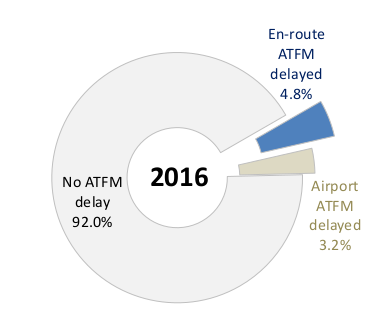
\includegraphics[width=0.8\textwidth]{./imagenes/introduccion/tiposRetrasos.png}
		\caption{causas posibles de retraso de un vuelo. \textit{Fuente: EUROCONTROL}}
		\label{fig: Causas posibles de retraso de un vuelo}
	\end{center}
\end{figure}

Durante las últimas décadas se han desarrollado varios modelos cuya finalidad es tratar de resolver (o al menos minimizar) los retrasos en vuelos. Aunque los primeros estudios se centraron más en el modelo estadounidense, y por tanto trataban de resolver el cuello de botella de sus aeropuertos, recientemente también se han hecho estudios europeos más centrados en la saturación del espacio aéreo: 
\begin{enumerate}
	\item \textbf{Singe-Airport Ground-Holding Problem (SAGHP):} poco utilizada a excepción de algunos aeropuertos italianos, este modelo tiene en cuenta el número de despegues y aterrizajes que puede soportar un aeropuerto por unidad de tiempo.
	\item \textbf{Multi-Airport Ground-Holding Problem (MAGHP): }muy similar al anterior, salvo que maneja varios aeropuertos de forma conjunta, teniendo en cuenta las relaciones entre ellos.
	\item \textbf{Air Traffic Flow Management Problem (ATFMP)}: introduce en el modelo el espacio aéreo. Como se puede ver en la figura \ref{fig: Causas posibles de retraso de un vuelo}, el porcentaje de retrasos en ruta fue mayor que el retraso en tierra. Esto se debe a que si un determinado espacio aéreo no está disponible (por sobresaturación, causas meteorológicas, etc), solo se verán afectados los vuelos cuya ruta estaba programada por ese sector.\\
	Sin embargo, la saturación de un aeropuerto ocasiona un retraso en cadena, afectando a todos los vuelos que iban a despegar o aterrizar en dicho aeropuerto.
	\begin{figure}[h]
		\begin{center}
			\centering
			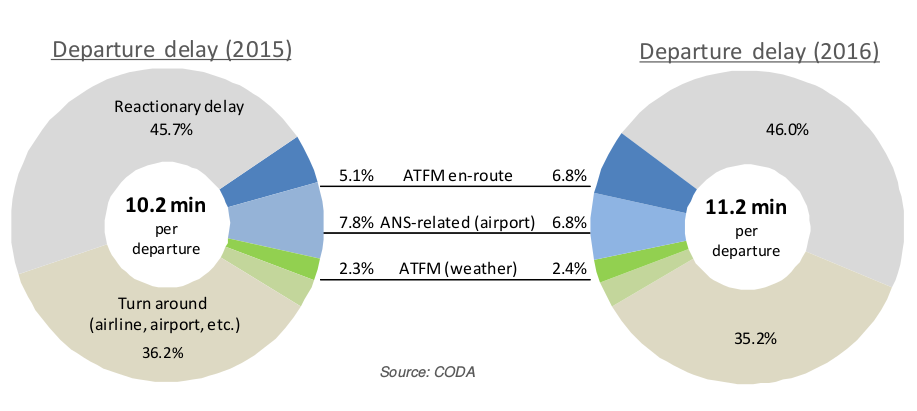
\includegraphics[width=0.8\textwidth]{./imagenes/introduccion/retrasosSalida.png}
			\caption{Comparativa retrasos 2015-2016. \textit{Fuente: EUROCONTROL}}
			\label{fig: Comparativa retrasos 2015-2016}
		\end{center}
	\end{figure}
	\item \textbf{Air Traffic Flow Management Rerouting Problem (ATFMRP): }muy similar a ATFMP, pero añade además la posibilidad de desviar vuelos.
	\begin{figure}[h]
		\begin{center}
			\centering
			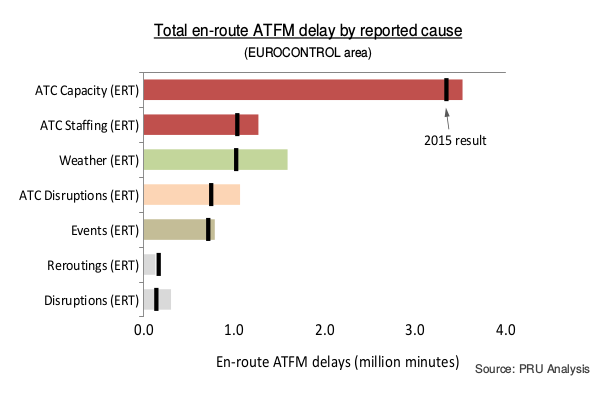
\includegraphics[width=0.8\textwidth]{./imagenes/introduccion/rerouting.png}
			\caption{Motivos de retrasos en 2016. \textit{Fuente: EUROCONTROL}}
			\label{fig: Retrasos en 2016}
		\end{center}
	\end{figure}
	\item \textbf{Air Traffic Flow Management Rerouting with Flight Cancellation Problem (ATFMRCP): }añade la posibilidad de cancelar vuelos. Se trata de un modelo más teórico que práctico, ya que la opción de cancelar vuelos no es una opción válida para casos reales.
\end{enumerate}


\section{Versiones anteriores}
Este Trabajo Final de Grado es la continuación del trabajo que llevaron a cabo Diego Ruiz Aguado y Gonzalo Quevedo García en 2012 en sus Proyectos Finales de Carrera, los cuales se apoyaron a su vez en la Tesis Doctoral de Alba Agustín  Martín (2011).\\
A continuación se hace una breve descripción del trabajo de  Diego Ruiz Aguado y Gonzalo Quevedo García:
\begin{enumerate}
	\item Los datos del problema se encontraban en una base de datos no relacional con redundancias. El primer paso consistió en migrar esta base de datos no relacional a una base de datos MySQL relacional y bien estructurada.
	\item Para obtener los datos que necesitaba el problema, se realizó un programa en java que se conectaba a la BBDD y creaba varios ficheros .txt en la que se volcaba toda la información necesaria para el posterior modelado del problema.
	\item A continuación, el programa en java leía estos ficheros .txt y creaba las estructuras de datos necesarias (árbol de rutas, vuelos, waypoints, etc).
	\item Posteriormente una subrutina en C se encargaba de definir un problema de CPLEX con la función objetivo y las restricciones necesarias.
	\item Finalmente, se ejecutaba el problema de optimización mediante la librería CPLEX para obtener la mejor solución del problema.
\end{enumerate}

Una vez seleccionado el vuelo al que se le iba a encontrar solución, el algoritmo CPLEX se encargaba de buscar una solución factible. A continuación se explica brevemente el funcionamiento de la librería de optimización:

\subsubsection{CPLEX}
CPLEX es una librería de optimización actualmente propiedad de IBM implementada en el lenguaje de programación C. CPLEX permite modelar un problema de optimización definiendo la función objetivo y todas las restricciones.\\
En la versión del problema de 2012 se utilizaba de la siguiente manera:
\begin{enumerate}
	\item Creación del modelo: mediante los ficheros .txt que contenían la información de la base de datos del problema se obtienen los nodos, arcos, restricciones y función objetivo del problema.
	\item Se optimiza el problema mediante CPLEX, del que obtendremos el valor final de la función objetivo
\end{enumerate}



\section{Nuevos objetivos}
La versión anterior del problema adolecía de un importante inconveniente: la función que se encargaba de tratar de encontrar la solución factible para cada vuelo se basaba en una función voraz \footnote{Un algoritmo voraz es aquel que sigue una heurística consistente en elegir la opción óptima en cada iteración para encontrar la mejor solución dado un determinado problema.}, por lo que el problema no podía salir de los máximos locales. De esta forma, el resultado del problema dependía en gran medida del orden en que se intentara encontrar una solución para cada vuelo.\\



Por tanto los objetivos marcados para este Trabajo de Fin de Grado han sido los siguientes (ordenados en decreciente prioridad):
\begin{enumerate}
	\item \textbf{Mejorar heurístico: }el objetivo principal de este TFG consiste en sustituir el algoritmo voraz por un heurístico que permita al problema escapar de los máximos locales, y por tanto aumentar en gran medida la calidad de la solución encontrada.
	\item \textbf{Desacoplar el programa de CPLEX y nueva estructura: }con la implementación de los nuevos heurísticos no es necesaria la librería de optimización. Se pasará de un sistema clásico de optimización (función objetivo y restricciones) a una estructura de objetos que permitan un manejo óptimo de las estructuras de datos durante la ejecución del algoritmo.
	\item \textbf{Mejorar el sistema de lectura de datos: }la versión actual del programa crea ficheros .txt en los que se vuelca toda la A2 del problema (vuelos, waypoints, rutas, etc) que pueden superar las 100.000 lineas. Estos ficheros auxiliares pueden sustituirse por ficheros mucho más pequeños en los que se exporta la información de la base de datos, y de forma interna el problema se encarga de crear las estructuras necesarias. De esta forma se reduce en gran medida el tiempo de creación del modelo del problema, además de obtener un módulo de lectura de datos exportable y fácilmente entendible.
	\item \textbf{Representación gráfica: }aunque estrictamente no aporta a mejorar la solución del problema, su representación gráfica puede ayudar a modelizar mejor el algoritmo, ya que permite visualizar de manera rápida y sencilla el estado del problema.
\end{enumerate}

Debido al enfoque teórico de este Trabajo de Fin de Grado, el modelo que se va a implementar se basa en el ATFMRCP, ya que permitirá cancelaciones, retrasos en aeropuertos, retrasos en ruta, y desvíos. 